%!TEX root = ../main.tex

\clearpage

\section{Implementation of MobilityDB Functions}
\label{section:general_functions}

The main focus of this master thesis is extending MobilityDB by adding a new type to represent moving regions and by implementing a set of functions to input, manipulate and output this new type. In Section \ref{section:mobilitydb_functions}, different types of functions and operators are presented, and most of these functions are polymorphic, meaning that they accept different input types and that their output depends on these input types. The next section lists and describes most of these functions, and explains how they are used to manipulate the tgeometry type.

\subsection{Type Declaration Functions and Parameters}
\label{section:type_declaration}

When defining a new SQL type, 2 functions have to be declared, and a few other functions and parameters are optional. The two required functions are \textit{input} and \textit{output}, converting a \textit{cstring} (C string type) to the newly declared type and back. The optional functions and parameters are used to declare the internal storage length of the type, the storage alignment in bytes, input/out to and from byte format, type modifier specification, and more.

As explained previously, two new types have been added to MobilityDB: \textit{rtransform} and \textit{tgeometry}. Four variations of the tgeometry type (\textit{tgeometryinst}, \textit{tgeometryi}, \textit{tgeometryseq} and \textit{tgeometrys}) are also present at the C-level, but only these two top-level types are exposed at the SQL level. Table \ref{table:rtransform_type_declaration} lists the declared parameters and functions for the rtransform type, and Table \ref{table:tgeometry_type_declaration} described the tgeometry type.

\begin{table}[h!]
    \centering
    \begin{tabularx}{\textwidth}{|l|l|X|}
    \hline
    \textbf{Parameter}  & \textbf{Value}        & \textbf{Description} \\ 
    \hline
    internal length     & 24                    & Internal storage length in bytes. \\
    \hline
    alignment           & double                & Storage alignment of the type. \\
    \hline
    \multicolumn{2}{|l|}{\textbf{Function}}     & \textbf{Description} \\ 
    \hline
    \multicolumn{2}{|l|}{input}                 & Conversion from \textit{cstring} to \textit{rtransform} type \\
    \hline
    \multicolumn{2}{|l|}{output}                & Conversion from \textit{rtransform} to \textit{cstring} type \\
    \hline
    \multicolumn{2}{|l|}{receive}               & Conversion from \textit{bytea} to \textit{rtransform} type \\
    \hline
    \multicolumn{2}{|l|}{send}                  & Conversion from \textit{rtransform} to \textit{bytea} type \\
    \hline
    \end{tabularx}
    \caption{Declared parameters and functions for the \textit{rtransform} type}
    \label{table:rtransform_type_declaration}
\end{table}

The rtransform type stores three double (8-byte) values, two for the translation and one for the rotation, and has thus a fixed length of 24 bytes. Since values of this type will never be store alone, but always as part of a tgeometry value, the storage strategy does not need to be declared. During the input from a string, we make sure that the value for the rotation is between $-\pi$ and $\pi$. The output as a string is formatted as follows:

\[
    \text{"RTransform(}\theta,\ v_x,\ v_y{)"}
\]

, where all three values are written with up to 15 decimal digits. The binary representation is simply a list of three doubles in the same order as in the string representation.

\begin{table}[h!]
    \centering
    \begin{tabularx}{\textwidth}{|l|l|X|}
    \hline
    \textbf{Parameter}  & \textbf{Value}        & \textbf{Description} \\ 
    \hline
    internal length     & variable              & Internal storage length of the type in bytes. \\
    \hline
    storage             & extended              & Storage strategy of the type. \\
    \hline
    alignment           & double                & Storage alignment of the type. \\
    \hline
    \multicolumn{2}{|l|}{\textbf{Function}}     & \textbf{Description} \\ 
    \hline
    \multicolumn{2}{|l|}{input}                 & Conversion from \textit{cstring} to \textit{tgeometry} type \\
    \hline
    \multicolumn{2}{|l|}{output}                & Conversion from \textit{tgeometry} to \textit{cstring} type \\
    \hline
    \multicolumn{2}{|l|}{receive}               & Conversion from \textit{bytea} to \textit{tgeometry} type \\
    \hline
    \multicolumn{2}{|l|}{send}                  & Conversion from \textit{tgeometry} to \textit{bytea} type \\
    \hline
    \end{tabularx}
    \caption{Declared parameters and functions for the \textit{tgeometry} type}
    \label{table:tgeometry_type_declaration}
\end{table}

The tgeometry type contains PostGIS polygons (which are of variable length) and can have an arbitrary number of defined instants, so it must be defined as variable-length. Since the type is variable in length, the \textit{plain} storage strategy, storing the values in-line without compression, cannot be used. The \textit{extended} strategy is thus used to compress large values, and even move them out of the main table if the value is still too large.

The string representation of the the tgeometry types depends on the duration of the value as described in Section \ref{section:mobilitydb} (instant, instant set, ...), and represents the values of the instants as PostGIS polygon types. These conversion functions from and to a string are defined together with the conversion functions from and to a byte list.

\subsection{Constructors}
\label{section:constructors}

Four different constructors exist for tgeometry types, one for each duration.

\begin{table}[h!]
    \centering
    \begin{tabularx}{\textwidth}{|l|X|}
    \hline
    \textbf{Function}   & \textbf{Signature} \\ 
    \hline
    tgeometryinst       & geometry(Polygon) x timestamptz $\rightarrow$ tgeometry(Instant) \\
    \hline
    tgeometryi          & array tgeometry(Instant) $\rightarrow$ tgeometry(Instant Set) \\
    \hline
    tgeometryseq        & array tgeometry(Instant) x lower inclusive x upper inclusive x linear $\rightarrow$ tgeometry(Sequence) \\
    \hline
    tgeometrys          & array tgeometry(Sequence) $\rightarrow$ tgeometry(Sequence Set) \\
    \hline
    \end{tabularx}
    \caption{Constructor functions}
    \label{table:constructor_funcs}
\end{table}

When creating a tgeometryinst, the input geometry is checked to make sure that it is a 2D polygon. Both the instant set and sequence constructors receive and array of tgeometryinst as input, while the sequence set constructor requires an array of tgeometryseq. Different checks are done to make sure that this input array corresponds to a correct temporal geometry.

First of all, when creating an instance set or a sequence, the usual timestamp checks are done, meaning that the instants must have strictly increasing timestamps. Lastly, the regions are compared with one another, to make sure that they have the same shape.

This comparison between regions is done in two steps. A first quick check compares the number of inner rings of the polygons and if both polygons have the same number of rings, it compares the number of points on each ring. If two polygons are able to pass this check, the transformation between the two polygons is computed from the first two points of the outer ring of both polygons, and the transformation is then applied to one of the polygons. Only polygons where the corresponding points are close enough to each other (their distance is smaller than a fixed $\epsilon$) after the transformation are considered fixed-shape. Figure \ref{fig:constr_checks} shows examples of polygons that fail the first test (a), pass the first test, but fail the second (b), or pass all tests because they are indeed fixed-shape (c).

\begin{figure}[h!]
    \centering
    \begin{subfigure}{.3\textwidth}
        \centering
        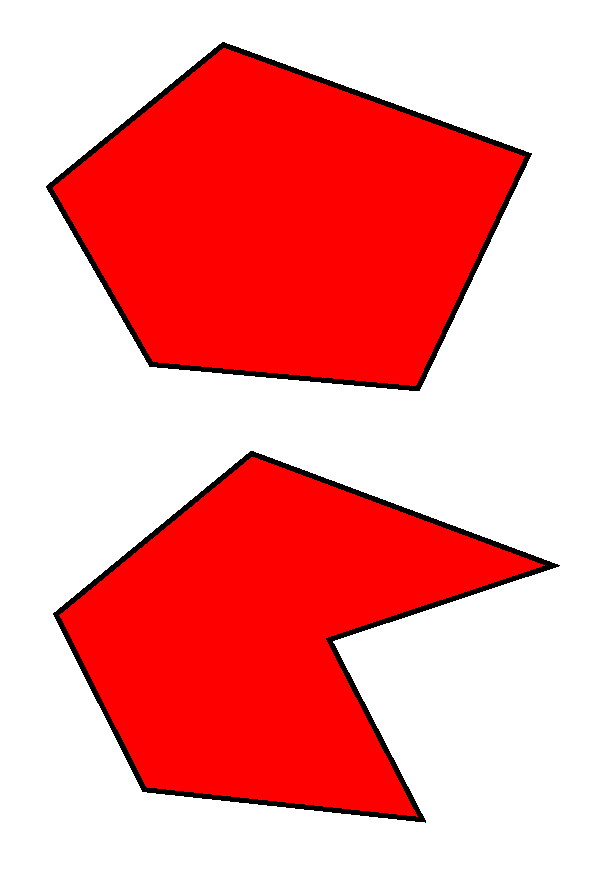
\includegraphics[width=\textwidth]{images/fail_first_test.pdf}
        \caption{Different number of vertices}
    \end{subfigure}
    \hfill
    \begin{subfigure}{.3\textwidth}
        \centering
        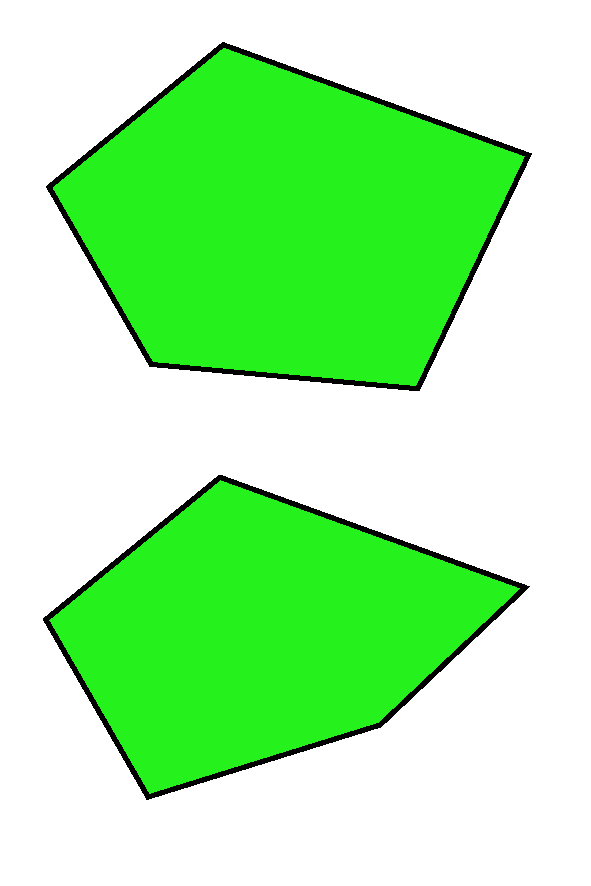
\includegraphics[width=\textwidth]{images/fail_second_test.pdf}
        \caption{Different shape}
    \end{subfigure}
    \hfill
    \begin{subfigure}{.3\textwidth}
        \centering
        \includegraphics[width=\textwidth]{images/pass_all_tests.pdf}
        \caption{Same shape, only transformed}
    \end{subfigure}
    \caption{Polygons failing or passing the different constructor checks}
    \label{fig:constr_checks}
\end{figure}

If all polygons are indeed fixed-shape, the input array is accepted and saved using the representation described in Section \ref{section:internal_repr_i} and \ref{section:internal_repr_seq}.

The sequence constructor has three additional parameters. The first two specify if the start and end instant are inclusive or not and by default both are considered inclusive. The last parameter specifies the interpolation strategy for the sequence, either linear or stepwise. The sequence set constructor has checks similar to the two previous ones, but since the input durations are already assumed to be sequences, only the comparisons between distinct sequences has to be done. During these comparisons, checks are done to assure continuously increasing timestamps, and fixed-shape polygons across the whole sequence set.

Every tgeometry instance of either instant set, sequence or sequence set duration also computes and saves a bounding box used for optimization purposes. Section \ref{section:bbox_funcs} lists a few bounding-box specific functions, and Section \ref{section:bbox} explains how these bounding boxes can be computed. Temporal points of sequence and sequence set duration also save a \textit{trajectory}, which is also used to optimize a few functions. The polygon equivalent of this trajectory is the \textit{traverser area} of the polygon. The computation of the traversed areas of a moving region is discussed in Section \ref{section:traversed_area}.

Lastly, the arrays of instants and sequences stored are normalize during the input process to allow for efficient comparisons later on. This normalization is necessary to ensure that identical paths have the same internal representation. This topic is further discussed in Section \ref{section:normalization}.

\subsection{Transformation Functions}
\label{section:transformation_funcs}

Table \ref{table:transformation_funcs} lists the transformations functions that can be applied to tgeometry objects. The first four transformation functions are used to change the duration of a temporal geometry. These transformations are only possible when the correct number of instants and/or sequences are present in the input tgeometry. For example, for a temporal geometry to be transformed into a tgeometryinst, it must contain a single instant. Transforming into an instant set from a sequence set is only possible if every sequence in the set contains a single instant. The six possible transformations are listed below.

\begin{itemize}
    \item Instant $'\mathcal{R}@t'$ $\leftrightarrow$ Instant Set $'\{\mathcal{R}@t\}'$
    \item Instant $'\mathcal{R}@t'$ $\leftrightarrow$ Sequence $'[\mathcal{R}@t]'$
    \item Instant $'\mathcal{R}@t'$ $\leftrightarrow$ Sequence Set $'\{[\mathcal{R}@t]\}'$
    \item Instant Set $'\{\mathcal{R}@t\}'$ $\leftrightarrow$ Sequence $'[\mathcal{R}@t]'$
    \item Instant Set $'\{\mathcal{R}_0@t_0,\ ...,\ \mathcal{R}_n@t_n\}'$ $\leftrightarrow$ Sequence Set $'\{[\mathcal{R}_0@t_0],\ ...,\ [\mathcal{R}_n@t_n]\}'$
    \item Sequence $'[\mathcal{R}_0@t_0,\ ...,\ \mathcal{R}_n@t_n]'$ $\leftrightarrow$ Sequence Set $'\{[\mathcal{R}_0@t_0,\ ...,\ \mathcal{R}_n@t_n]\}'$
\end{itemize}

Next to changing their duration, temporal geometries can also be transformed by appending a new instant to the end or by merging two temporal geometries together, during which similar checks as in the constructors are applied.

\begin{table}[h!]
    \centering
    \begin{tabularx}{\textwidth}{|l|X|}
    \hline
    \textbf{Function}   & \textbf{Signature} \\ 
    \hline
    tgeometryinst       & tgeometry $\rightarrow$ tgeometry(Instant) \\
    \hline
    tgeometryi          & tgeometry $\rightarrow$ tgeometry(Instant Set) \\
    \hline
    tgeometryseq        & tgeometry $\rightarrow$ tgeometry(Sequence) \\
    \hline
    tgeometrys          & tgeometry $\rightarrow$ tgeometry(Sequence Set) \\
    \hline
    \hline
    appendInstant       & tgeometry x tgeometry(Instant) $\rightarrow$ tgeometry \\
    \hline
    merge               & tgeometry x tgeometry $\rightarrow$ tgeometry \\
    \hline
    merge               & array tgeometry $\rightarrow$ tgeometry \\
    \hline
    \end{tabularx}
    \caption{Transformation functions}
    \label{table:transformation_funcs}
\end{table}

\subsection{Accessors}
\label{section:accessors}

A large list of accessor functions exist to retrieve the duration, memory size, individual values, instants, timestamps and more. (Table \ref{table:accessor_funcs})

\begin{table}[h!]
    \centering
    \begin{tabularx}{\textwidth}{|l|X|}
    \hline
    \textbf{Function}   & \textbf{Signature} \\ 
    \hline
    duration            & tgeometry $\rightarrow$ text\\
    \hline
    interpolation       & tgeometry $\rightarrow$ text\\
    \hline
    memSize             & tgeometry $\rightarrow$ integer \\
    \hline
    getValue            & tgeometry(Instant) $\rightarrow$ geometry(Polygon) \\
    \hline
    startValue          & tgeometry $\rightarrow$ geometry(Polygon) \\
    \hline
    endValue            & tgeometry $\rightarrow$ geometry(Polygon) \\
    \hline
    getTimestamp        & tgeometry(Instant) $\rightarrow$ timestamptz \\
    \hline
    getTime             & tgeometry $\rightarrow$ periodset \\
    \hline
    timespan            & tgeometry $\rightarrow$ interval \\
    \hline
    shift               & tgeometry $\rightarrow$ tgeometry \\
    \hline
    num*                & tgeometry $\rightarrow$ integer \\
    \hline
    start*              & tgeometry $\rightarrow$ * \\
    \hline
    end*                & tgeometry $\rightarrow$ * \\
    \hline
    *N                  & tgeometry x integer $\rightarrow$ *\\
    \hline
    *s                  & tgeometry $\rightarrow$ array *\\
    \hline
    \end{tabularx}
    \caption{Accessor functions}
    \label{table:accessor_funcs}
\end{table}

\textit{Duration} returns one of $\{$\textit{Instant}, \textit{Instant Set}, \textit{Sequence}, \textit{Sequence Set}$\}$, \textit{interval} returns either \textit{Discrete} for instants and instant set, or one of $\{$\textit{Linear}, \textit{Stepwise}$\}$ for sequences and sequence sets, and \textit{memsize} returns the internal memory size in bytes.

Other accessor functions are defined to retrieve individual values, timestamps or sequences from the temporal geometry. In Table \ref{table:accessor_funcs}, all functions containing the symbol '*' are part of a set of functions returning a certain type of element. These functions return the number of that element in the tgeometry, the first, last or Nth element, and an array containing all elements respectively. This set is defined for the \textit{Timestamp}, \textit{Instant} and \textit{Sequence} elements. A complete list of these functions can be found in Appendix \ref{appendix:complete_funct_tables}.

\subsection{Always/Ever Comparison}
\label{section:always_ever}

The following functions and operators compare a temporal geometry with a fixed region value (Polygon), and return the result of the \textit{ever equals}, \textit{always equals}, \textit{ever not equals} or \textit{always not equals} comparisons. \\

% Ex: Always equals:
% \begin{empheq}[box=\mygreybox]{flalign*}
%     & \text{SELECT tgeometry }'\{\text{Polygon}((0 0, 1 0, 1 1, 0 1, 0 0))@\text{2001-01-01}\}'\ \%=    & \\
%     & \eqtab\text{geometry } '\text{Polygon}((0 0, 1 0, 1 1, 0 1, 0 0))';                               & \\
%     & \text{- - true}                                                                                   &
% \end{empheq}

\begin{table}[h!]
    \centering
    \begin{tabularx}{\textwidth}{|l|l|X|}
    \hline
    \textbf{Function}   & \textbf{Operator} & \textbf{Signature} \\
    \hline
    ever\_eq    & $?=$      & tgeometry x geometry(Polygon) $\rightarrow$ boolean \\
    \hline
    always\_eq  & $\%=$     & tgeometry x geometry(Polygon) $\rightarrow$ boolean \\
    \hline
    ever\_ne    & $\&<>$    & tgeometry x geometry(Polygon) $\rightarrow$ boolean \\
    \hline
    always\_ne  & $\%<>$    & tgeometry x geometry(Polygon) $\rightarrow$ boolean \\
    \hline
    \end{tabularx}
    \caption{Always/Ever comparison functions and operators}
    \label{table:always_ever_funcs}
\end{table}

\subsection{Restriction and Difference Functions}
\label{section:restriction_and_difference}

These functions are used to restrict a temporal geometry to a given value (restriction functions), or to the complement of that value (difference functions). The given value can range from a single region (Polygon) value to a timestamp, or even a set of period values. The full set of restriction functions is listed in Table \ref{table:restriction_funcs}, and Table \ref{table:diff_funcs} lists the difference functions.

\begin{table}[h!]
    \centering
    \begin{tabularx}{\textwidth}{|l|X|}
    \hline
    \textbf{Function}   & \textbf{Signature} \\ 
    \hline
    atValue             & tgeometry x geometry $\rightarrow$ tgeometry\\
    \hline
    atValues            & tgeometry x array geometry $\rightarrow$ tgeometry\\
    \hline
    atTimestamp         & tgeometry x timestamptz $\rightarrow$ tgeometry \\
    \hline
    atTimestampSet      & tgeometry x timestampset $\rightarrow$ tgeometry \\
    \hline
    atPeriod            & tgeometry x period $\rightarrow$ tgeometry \\
    \hline
    atPeriodSet         & tgeometry x periodset $\rightarrow$ tgeometry \\
    \hline
    \end{tabularx}
    \caption{Restriction functions}
    \label{table:restriction_funcs}
\end{table}

For example, if we want to remove the data in a temporal geometry between to given timestamps, we can use the \textit{minusPeriod} function with as second argument a period starting at the first and ending at the second timestamp.

\begin{table}[h!]
    \centering
    \begin{tabularx}{\textwidth}{|l|X|}
    \hline
    \textbf{Function}   & \textbf{Signature} \\ 
    \hline
    minusValue             & tgeometry x geometry $\rightarrow$ tgeometry\\
    \hline
    minusValues            & tgeometry x array geometry $\rightarrow$ tgeometry\\
    \hline
    minusTimestamp         & tgeometry x timestamptz $\rightarrow$ tgeometry \\
    \hline
    minusTimestampSet      & tgeometry x timestampset $\rightarrow$ tgeometry \\
    \hline
    minusPeriod            & tgeometry x period $\rightarrow$ tgeometry \\
    \hline
    minusPeriodSet         & tgeometry x periodset $\rightarrow$ tgeometry \\
    \hline
    \end{tabularx}
    \caption{Difference functions}
    \label{table:diff_funcs}
\end{table}

\subsection{Comparison Operators}
\label{section:comparison_funcs}

A set of comparison operators is defined in PostgreSQL, and they have been extended to accept arguments of type temporal geometry. In practice, only the $=$ (equals) and $<>$ (not equals) operators are useful for real-world applications, but the other operators are used internally to create B-tree indexes on the tgeometry type.

\begin{table}[h!]
    \centering
    \begin{tabularx}{\textwidth}{|l|l|X|}
    \hline
    \textbf{Function}   & \textbf{Operator} & \textbf{Signature} \\
    \hline
    tgeometry\_lt    & $<$   & tgeometry x tgeometry $\rightarrow$ boolean \\
    \hline
    tgeometry\_le    & $<=$   & tgeometry x tgeometry $\rightarrow$ boolean \\
    \hline
    tgeometry\_eq    & $=$   & tgeometry x tgeometry $\rightarrow$ boolean \\
    \hline
    tgeometry\_ne    & $<>$   & tgeometry x tgeometry $\rightarrow$ boolean \\
    \hline
    tgeometry\_ge    & $>=$   & tgeometry x tgeometry $\rightarrow$ boolean \\
    \hline
    tgeometry\_gt    & $>$   & tgeometry x tgeometry $\rightarrow$ boolean \\
    \hline
    tgeometry\_cmp    & & tgeometry x tgeometry $\rightarrow$ integer \\
    \hline
    \end{tabularx}
    \caption{Comparison functions and operators}
    \label{table:comparison_funcs}
\end{table}

\subsection{Temporal Comparison Operators}
\label{section:temporal_comparison}

The previous equality and inequality operators returned a single boolean value, but we might also be interested in knowing when two temporal geometries are equal or when they differ as a function of time. The following two operators return a temporal bool representing the result over time of the equality or inequality operator on the input values.

\begin{table}[h!]
    \centering
    \begin{tabularx}{\textwidth}{|l|l|X|}
    \hline
    \textbf{Function}   & \textbf{Operator} & \textbf{Signature} \\
    \hline
    tgeo\_eq    & $\#=$   & \{tgeometry, geometry(Polygon)\} x \{tgeometry, geometry(Polygon)\} $\rightarrow$ tbool \\
    \hline
    tgeo\_ne    & $\#<>$  & \{tgeometry, geometry(Polygon)\} x \{tgeometry, geometry(Polygon)\} $\rightarrow$ tbool \\
    \hline
    \end{tabularx}
    \caption{Comparison functions and operators}
    \label{table:comparison_funcs}
\end{table}

\subsection{Spatial Functions}
\label{section:spatial_funcs}

As has been done for the temporal points previously in MobilityDB (briefly described in Section \ref{section:mobilitydb_functions}), multiple spatial functions similar to those defined in PostGIS are exposed. 

Table \ref{table:spatial_funcs} shows a non-exhaustive list of spatial functions that can be applied to the tgeometry type.

\begin{table}[h!]
    \centering
    \begin{tabularx}{\textwidth}{|l|X|}
    \hline
    \textbf{Function}   & \textbf{Signature} \\ 
    \hline
    traversed\_area      & tgeometry $\rightarrow$ geometry(Polygon)\\
    \hline
    centroid            & tgeometry $\rightarrow$ tgeompoint\\
    \hline
    rotation\_speed      & tgeometry $\rightarrow$ tfloat \\
    \hline
    nearestApproachDistance & \{tgeometry, geometry(Polygon)\} x \{tgeometry, geometry(Polygon)\} $\rightarrow$ float \\
    \hline
    nearestApproachInstant  & \{tgeometry, geometry(Polygon)\} x \{tgeometry, geometry(Polygon)\} $\rightarrow$ tgeometry(Instant) \\
    \hline
    shortestLine         & \{tgeometry, geometry(Polygon)\} x \{tgeometry, geometry(Polygon)\} $\rightarrow$ geometry(LineString) \\
    \hline
    distance         & \{tgeometry, geometry(Polygon)\} x \{tgeometry, geometry(Polygon)\} $\rightarrow$ tfloat \\
    \hline
    \end{tabularx}
    \caption{Spatial functions}
    \label{table:spatial_funcs}
\end{table}

The \textit{traversed area} function returns a polygon representing the area traversed by the moving region. The computation of this area is described in Section \ref{section:traversed_area}.

\textit{Centroid} is a variant of the \textit{ST\_Centroid} PostGIS function, returning the evolution of the centroid of a temporal region. Since in our case the centroid is assumed to be the center of rotation, it moves linearly between two defined instants, and a temporal point containing the position of the centroid of a temporal region can thus be easily computed and returned.

Computing the translation or rotation speed of a polygon can also be of interest, but since the translation speed can be retrieved by applying the \textit{speed} function (defined for temporal points) on the centroid of the moving region, only the rotation speed has to be handled. This is thus returned by the \textit{rotation\_speed} function, which returns a temporal float. Since we assume linear interpolation between instants, the rotation speed is assumed to be constants between to instants.

The four last functions return respectively the smallest distance possible between the two (temporal) regions, the instant from the first temporal region at which this distance was attained, a segment going from the first region to the second at their closest instant, and finally a temporal float representing the evolution of the distance between the two regions during their movement. 

The three first functions (\textit{nearestApproachDistance}, \textit{nearestApproachInstant} and \textit{shortestLine}) can be implemented easily if the \textit{distance} function exists. Indeed, if we have a tfloat value representing the result of the distance function applied to two (moving) regions, we can use already defined functions on the tfloat type to find the minimum value, or the instant at which this minimum value is obtained, which solves the first two problems. After computing the position of both regions when they were at their closest, we can then also use a PostGIS spatial function to compute the smallest line joining these polygons, which is the result of the third question.

This leaves us with the implementation of the \textit{distance} function, which, due to its complexity and time constraints, is left as future work.

\subsection{Bounding Box Functions and Operators}
\label{section:bbox_funcs}

Bounding boxes are precomputed for temporal geometries of instant set, sequence and sequence set duration. These boxes are used in multiple functions to prune some input values with fast checks applied before the function itself. For example, if we want to compute the instants at which two regions were within 5 meters of each other, we can first compute the minimum distance between the bounding boxed and return an empty value if this distance is larger than 5 meters.

Computing this bounding box is relatively tricky when the temporal geometry is a sequence or a sequence set, since the bounding box is not simply the union of the bounding boxes of all instants. Section \ref{section:bbox} explains how the bounding boxes of moving regions can be computed in two different ways.

Some bounding box operators are also exposed to the user . These operators are polymorphic and allow all types of input that can be casted into an spatio-temporal box (STbox). 

\begin{table}[h!]
    \centering
    \begin{tabularx}{\textwidth}{|l|l|X|}
    \hline
    \textbf{Function}   & \textbf{Operator} & \textbf{Signature} \\ 
    \hline
    stbox               & & tgeometry $\rightarrow$ stbox\\
    \hline
    expandSpatial       & & tgeometry x float $\rightarrow$ stbox\\
    \hline
    expandTemporal      & & tgeometry x interval $\rightarrow$ stbox \\
    \hline
    contains\_bbox      & $@>$ & \{tgeometry, geometry, stbox\} x \{tgeometry, geometry, stbox\} $\rightarrow$ stbox \\
    \hline
    contained\_bbox     & $<@$ & \{tgeometry, geometry, stbox\} x \{tgeometry, geometry, stbox\} $\rightarrow$ stbox \\
    \hline
    overlaps\_bbox      & $\&\&$ & \{tgeometry, geometry, stbox\} x \{tgeometry, geometry, stbox\} $\rightarrow$ stbox \\
    \hline
    same\_bbox          & $\sim=$ & \{tgeometry, geometry, stbox\} x \{tgeometry, geometry, stbox\} $\rightarrow$ stbox \\
    \hline
    adjacent\_bbox      & $-\mid-$ & \{tgeometry, geometry, stbox\} x \{tgeometry, geometry, stbox\} $\rightarrow$ stbox \\
    \hline
    \end{tabularx}
    \caption{Bounding box functions and operators}
    \label{table:bbox_funcs}
\end{table}
